\documentclass[10pt]{book}

% global setup
%-------------------------------------------------------------------------
% package manager
%-------------------------------------------------------------------------

% page layout
\usepackage[a4paper,top=4.0cm,textheight=22.0cm,textwidth=16.0cm]{geometry}
\usepackage{fancyhdr,indentfirst,pdflscape,array,listings,longtable,titlesec}

% hyperlinks
\usepackage[xetex,colorlinks=true,linkcolor=purple,anchorcolor=blue,citecolor=green]{hyperref}

% reference
\usepackage[sort,super,comma,compress]{natbib}

% figure
\usepackage{graphicx,tikz,color}
\usetikzlibrary{snakes,arrows,mindmap,automata}

% math
\usepackage{textcomp,amsmath,amssymb,mathrsfs,marvosym,wasysym}

% font
\usepackage{fontspec,xunicode}

%-------------------------------------------------------------------------
% font style
%-------------------------------------------------------------------------

% need fontspec package support
\setmainfont{Times}
\setmonofont{Lucida Sans Typewriter}

%-------------------------------------------------------------------------
% page format
%-------------------------------------------------------------------------

% define header and footer
\pagestyle{fancy}
\fancyhf{}
\renewcommand{\chaptermark}[1]{\markboth{\emph{#1}}{}}
\renewcommand{\sectionmark}[1]{\markright{\thesection\ #1}}
\fancyhead[LE,RO]{\thepage}
\fancyhead[RE]{\leftmark}
\fancyhead[LO]{\rightmark}
%\fancyfoot[LE,RO]{by lihuang}
\renewcommand{\headrulewidth}{0.4pt}
\renewcommand{\footrulewidth}{0.4pt}
\fancypagestyle{plain}{
 	\fancyhf{}
	\renewcommand{\headrulewidth}{0pt}
	\renewcommand{\footrulewidth}{0pt}
}

% redefine \clearpage
\makeatletter
\def\cleardoublepage{\clearpage\if@twoside \ifodd\c@page\else
    \hbox{}
    \thispagestyle{plain}
    \newpage
    \if@twocolumn\hbox{}\newpage\fi\fi\fi}
\makeatother \clearpage{\pagestyle{plain}\cleardoublepage}

%% define line spacing
\renewcommand{\baselinestretch}{1.5}
\renewcommand{\arraystretch}{1.5}

%-------------------------------------------------------------------------
% chapter format
%-------------------------------------------------------------------------

\titleformat{\chapter}[display]
  {\bfseries\Large}
  {\filleft \Huge Chapter {\thechapter}}
  {4ex}
  {\titlerule
   \vspace{2ex}%
   \filright}
  [\vspace{2ex}%
   \titlerule]

%-------------------------------------------------------------------------
% equation format
%-------------------------------------------------------------------------

\renewcommand{\theequation}{\thechapter.\arabic{equation}}
%\renewcommand{\theequation}{\thesection.\arabic{equation}}

%-------------------------------------------------------------------------
% figure format
%-------------------------------------------------------------------------

\renewcommand{\thefigure}{\thechapter.\arabic{figure}}
%\renewcommand{\thefigure}{\thesection.\arabic{figure}}

%-------------------------------------------------------------------------
% self-defined commands
%-------------------------------------------------------------------------

\newcommand{\iqist}{ {\color{red}$i$}{\color{cyan}QIST} }
\newcommand{\azalea}{ {\color{red} $\mathcal{A}$zalea} }
\newcommand{\gardenia}{ {\color{violet} $\mathcal{G}$ardenia} }
\newcommand{\narcissus}{ {\color{blue} $\mathcal{N}$arcissus} }
\newcommand{\begonia}{ {\color{green} $\mathcal{B}$egonia} }
\newcommand{\lavender}{ {\color{orange} $\mathcal{L}$avender} }
\newcommand{\pansy}{ {\color{olive} $\mathcal{P}$ansy} }
\newcommand{\manjushaka}{ {\color{cyan} $\mathcal{M}$anjushaka} }
\newcommand{\daisy}{ {\color{lime} $\mathcal{D}$aisy} }
\newcommand{\jasmine}{ {\color{brown} $\mathcal{J}$asmine} }
\newcommand{\hibiscus}{ {\color{magenta} $\mathcal{H}$ibiscus} }


\begin{document}

% cover
%-------------------------------------------------------------------------
% title page 1
%-------------------------------------------------------------------------
{
\pagestyle{plain}
\parindent 0pt
\vbox{}

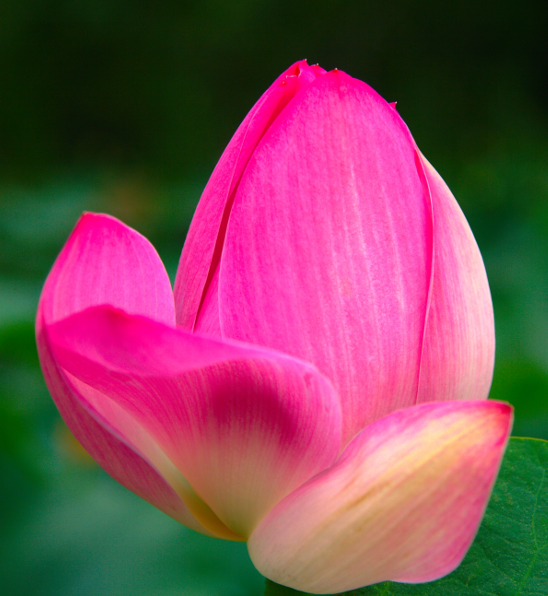
\includegraphics[width=5cm]{figure/cover.png}

\Huge{\textsf{Reference Manual for {\color{red}I}nteracting {\color{cyan}Q}uantum {\color{cyan}I}mpurity {\color{cyan}S}olver {\color{cyan}T}oolkit}}

\Large{\textsf{Draft Version \today}}

\Large{\textsf{Written by}:\\ \textbf{Li Huang}, \textbf{Yilin Wang}, \textbf{Zi Yang Meng}, and \textbf{Liang Du}}

\vbox{}
\clearpage

\huge{{\iqist} Developer Team}

\vspace{-1cm}
\rule{\textwidth}{1pt}

\Large{Core Developers:}

\Large{\textbf{Li Huang}$^{\dagger}$ and \textbf{Yilin Wang}$^{\ddagger}$}

\Large{Key Contributors:}

\Large{\textbf{Zi Yang Meng}$^{\ddagger, \flat}$ and \textbf{Liang Du}$^{\sharp}$}

\Large{Directors and Supervisors:}

\Large{\textbf{Philipp Werner}$^{\dagger}$ and \textbf{Xi Dai}$^{\ddagger}$}

\vskip 1.0cm
$^{\dagger}$\large{\textsf{Department of Physics, University of Fribourg, 1700 Fribourg, Switzerland}}

$^{\ddagger}$\large{\textsf{Beijing National Laboratory for Condensed Matter Physics, and \\ 
$^{\ }$Institute of Physics, Chinese Academy of Sciences, Beijing 100190, China}}

$^{\flat}$\large{\textsf{Department of Physics, University of Toronto, Toronto, Ontario M5S 1A7, Canada}}

$^{\sharp}$\large{\textsf{Department of Physics, The University of Texas at Austin, Austin, Texas 78712, USA}}

\vbox{}         
\clearpage
}

%-------------------------------------------------------------------------
% title page 2
%-------------------------------------------------------------------------
{
\pagestyle{plain}
\parindent 0pt
\vbox{}
\vskip 0pt plus 1fill
\textsf{To my lovely wife X. Zhao}
\vskip 1em
\hfill\emph{\textsf{L. H}}
\parindent 0pt
\vbox{}
\vskip 0pt plus 1fill
\textsf{To my lovely girlfriend X.Y. Mao}
\vskip 1em
\hfill\emph{\textsf{Y.L. Wang}}
\vskip 0pt plus 3fill

\parindent 0pt
\textsf{Copyright 2015 by Li Huang}

\medskip
\textsf{Permission is granted to copy, distribute and/or modify \emph{the documentation}
under the terms of the \textsc{gnu} Free Documentation License, Version 1.2
or any later version published by the Free Software Foundation;
with no Invariant Sections, no Front-Cover Texts, and no Back-Cover Texts.}

\medskip  
\textsf{Permission is granted to copy, distribute and/or modify \emph{the 
code of the package} under the terms of the \textsc{gnu} Public License, Version 2
or any later version published by the Free Software Foundation.}

\medskip  
\textsf{Permission is also granted to distribute and/or modify \emph{both
the documentation and the code} under the conditions of the LaTeX
Project Public License, either version 1.3 of this license or (at
your option) any later version.}

\vbox{}
\clearpage 
}


\frontmatter

% outlines
\tableofcontents

% figures
\listoffigures

% tables
\listoftables

\mainmatter
\pagestyle{fancy}

% main contents
\chapter{INTRODUCTION}
\section{What's {\iqist}?}
\section{Motivation}
\section{Software architecture}
\section{Main features}
\section{Development history}
\section{Policy and licences}

\chapter{INSTALLATION}
\section{Obtain}
\section{Uncompress}
\section{Direcrory structures}
\section{Compiling environment}
\section{Compiling system}
\section{Build impurity solvers}
\section{Build auxiliary tools}
\section{Build documents}
\section{Build application programming interfaces}

\chapter{RUNNING}
\section{Configure your system}
\section{Create input files}
\section{Execute codes}
\section{Monitor and Profile}

\chapter{STANDARD INPUT FILES}
\section{solver.ctqmc.in}
\section{solver.eimp.in}
\section{solver.hyb.in}
\section{solver.anydos.in}
\section{solver.ktau.in}
\section{atom.cix}

\chapter{STANDARD OUTPUT FILES}
\section{Terminal output}
\subsection{out.dat}
\section{File output}
\subsection{solver.green.dat}
\subsection{solver.green.bin}
\subsection{solver.weiss.dat}
\subsection{solver.hybrid.dat}
\subsection{solver.grn.dat}
\subsection{solver.wss.dat}
\subsection{solver.hyb.dat}
\subsection{solver.sgm.dat}
\subsection{solver.hub.dat}
\subsection{solver.nmat.dat}
\subsection{solver.schi.dat}
\subsection{solver.ochi.dat}
\subsection{solver.twop.dat}
\subsection{solver.vrtx.dat}
\subsection{solver.hist.dat}
\subsection{solver.prob.dat}
\subsection{solver.kernel.dat}
\subsection{solver.status.dat}

\chapter{PARAMETERS}
\section{isscf}
\section{issun}
\section{isspn}
\section{isbin}
\section{isort}
\section{isvrt}
\section{isscr}
\section{nband}
\section{nspin}
\section{norbs}
\section{ncfgs}
\section{nzero}
\section{nvect}
\section{nhmat}
\section{nfmat}
\section{niter}
\section{U}
\section{Uc}
\section{Uv}
\section{Jz}
\section{Js}
\section{Jp}
\section{lc}
\section{wc}
\section{mune}
\section{beta}
\section{part}
\section{alpha}
\section{lemax}
\section{legrd}
\section{chmax}
\section{chgrd}
\section{mkink}
\section{mfreq}
\section{nffrq}
\section{nbfrq}
\section{nfreq}
\section{ntime}
\section{nleja}
\section{npart}
\section{nflip}
\section{ntherm}
\section{nsweep}
\section{nwrite}
\section{nclean}
\section{nmonte}
\section{ncarlo}

\chapter{AUXILIARY TOOLS}
\section{{\jasmine} component}
\section{{\hibiscus} component}
\subsection{Maximum entropy method: entropy1}
\subsection{Maximum entropy method: entropy2}
\subsection{Stochastic analytical continuation: sac}
\subsection{Analytical continuation for self-energy: swing}
\subsection{toolbox/makechi}
\subsection{toolbox/makedos}
\subsection{toolbox/makekra}
\subsection{toolbox/makescr}
\subsection{toolbox/makesig}
\subsection{toolbox/makestd}
\subsection{toolbox/maketau}
\subsection{toolbox/makeups}
\subsection{script/pysci.py}
\subsection{script/check.py}
\section{Parquet component}

\chapter{APPLICATION PROGRAMMING INTERFACES}
\section{Fortran binding}
\section{Python binding}
\section{iqist.py}

\chapter{{\iqist} IN ACTION}
\section{Basic applications}
\subsection{Hello {\iqist}!}
\subsection{Mott metal-insulator transition}
\section{Advanced applications I: Complex systems}
\subsection{General Coulomb interaction}
\subsection{Spin-orbital coupling}
\subsection{Crystal field splitting}
\subsection{Retarded interaction and dynamical screening effect}
\section{Advanced applications II: Accurate measurement of physical observables}
\subsection{One-shot and self-consistent calculations}
\subsection{Data binning mode}
\subsection{Imaginary-time Green's function}
\subsection{Matsubara Green's function and self-energy function}
\subsection{Spin-spin correlation function and orbital-orbital correlation function}
\subsection{Two-particle Green's function and vertex function}
\section{Advanced applications III: post-processing procedures}
\subsection{Analytical continuation for imaginary-time Green's function}
\subsection{Analytical continuation for Matsubara self-energy function}
\section{Practical exercises}
\subsection{Orbital-selective Mott transition in two-band Hubbard model}
\subsection{Orbital Kondo and spin Kondo effects in three-band Anderson impurity model}

\chapter{INSIDE {\iqist}}
\section{Basic theory and methods}
\subsection{Quantum impurity model}
\subsection{Principles of continuous-time quantum Monte Carlo algorithm}
\subsection{Hybridization expansion}
\subsection{Physical observables}
\subsection{Two-particle measurements and DMFT + Parquet formalism}
\section{Implementations and optimizations}
\subsection{Development platform}
\subsection{Orthogonal polynomial representation}
\subsection{Improved estimator for the self-energy function}
\subsection{Random number generators}
\subsection{Subspaces and symmetry}
\subsection{Truncation approximation}
\subsection{Lazy trace evaluation}
\subsection{Divide-and-conquer and sparse matrix tricks}
\subsection{Parallelization}

\backmatter
\pagestyle{plain}

% appendix
% Appendix
{
\appendix
\chapter{Appendix}
\renewcommand\thesection{A.\arabic{section}}
\renewcommand{\theequation}{A.\arabic{equation}}
\renewcommand{\thefigure}{A.\arabic{figure}}

\section{TODO}

}


% reference
% reference

\addcontentsline{toc}{chapter}{\bibname}
\bibliographystyle{apsrev4-1}
\bibliography{bib/dmft}


\end{document}
